% Version 0.2
\section{Version 0.2}

The goal of this iteration and version was to create a \gls{MVP}. This \gls{MVP} contained what the team thought was the most important features of the application. It was done by creating an assumption with questions to be answered, select the the user stories needed to support that feature and measure the use.

\subsection{Assumption and questions}
The assumption to be confirmed for this iteration was
“Users want to add their books to the application using a barcode scanner”.

To confirm this assumption the team generated questions that should be answered to do so.
\begin{enumerate}
    \item Is it easy for the user to find a book’s barcode?
    \item Do the user think it is simple to scan a barcode?
\end{enumerate}


\subsection{Planning and design}
With the assumption and questions as basis, the team had to decide how to measure the result, and what user stories should be selected to be able to test the questions. After meeting with employees from Netlight, it was decided that user tests with paper prototypes was the best way to get an indication on whether our assumption was correct, and verify that our design was user friendly and intuitive. The user stories selected are described in section \ref{user-stories-v2}. 

An employee at Netlight named Magnus Skaalsveen had a session with the team where he taught the use of Lean UX.\cite{lean-ux} The goal of Lean UX is to create low-fidelity prototypes, like a whiteboard sketch or a paper prototype which take shot time to iterate upon. With these levels of design the build-measure-learn cycle can be executed more rapidly.  

At the meeting the team and Skaalsveen did a couple of sketches on a whiteboard to generate the design of the selected functionality. By doing so the team learned that there were a lot of points where the idea of the application still was unclear, and that by drawing in that manner created a good space to discuss those issues. 

Based on the sketches created on the whiteboard, paper prototypes were created to perform usability test where the goal was get indications on both questions and design.
The usability tests were performed at the university, and in the fashion of hallway tests executed on randomly selected students. Students were targeted because they were a part of the target audience and easy to come in contact with. 

 The tests would consist of a set of tasks the user would perform on paper prototypes of the application. The test team consisted of two team members. One acted as test leader and system while the other documented all the users feedback, hesitations, problems and other relevant information. After the test, a short unstructured interview was performed to ask what the user thought about the general idea behind the application. 

Prototypes created to support the selected user stories are shown in figure \ref{fig:user-story-prototype-v2-1} and \ref{fig:user-story-prototype-v2-2}.
In addition there were some design alternatives associated with user story number \ref{02-user-story-see-books-in-shelf}, the shelf view. The alternatives are shown in figure \ref{fig:design-alternatives-v2}. After the usability tests the first alternative was chosen as the design for the application. 

\begin{figure}
\centering
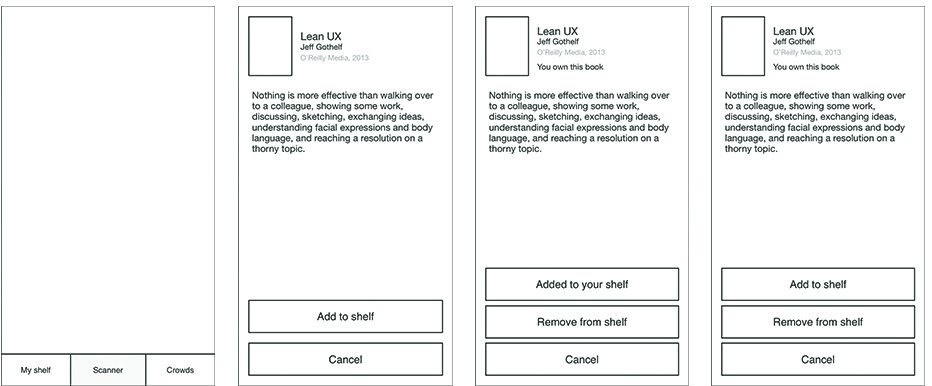
\includegraphics[height=5cm]{figs/v02/userstory-v2-1.jpg}
\caption{Paper prototype from the user stories of adding a book and scanning the barcode. }
\label{fig:user-story-prototype-v2-1}
\end{figure}

\begin{figure}
\centering
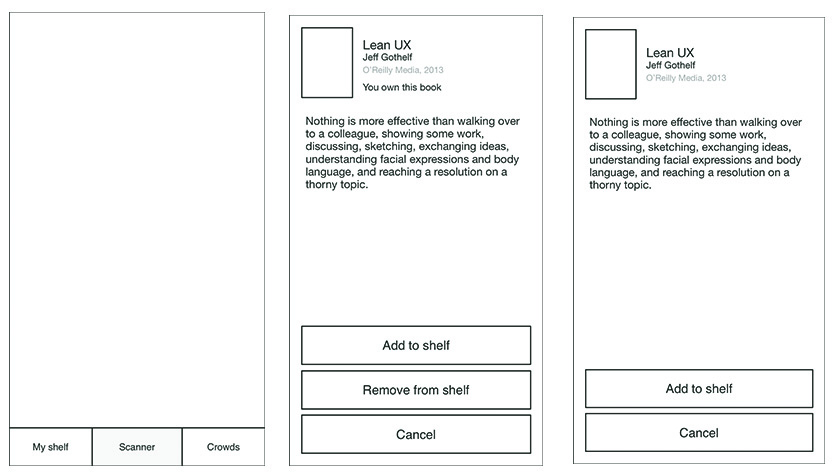
\includegraphics[height=5cm]{figs/v02/userstory-v2-2.jpg}
\caption{Paper prototype from the user stories of removing a book and scanning the barcode }
\label{fig:user-story-prototype-v2-2}
\end{figure}

\begin{figure}
\centering
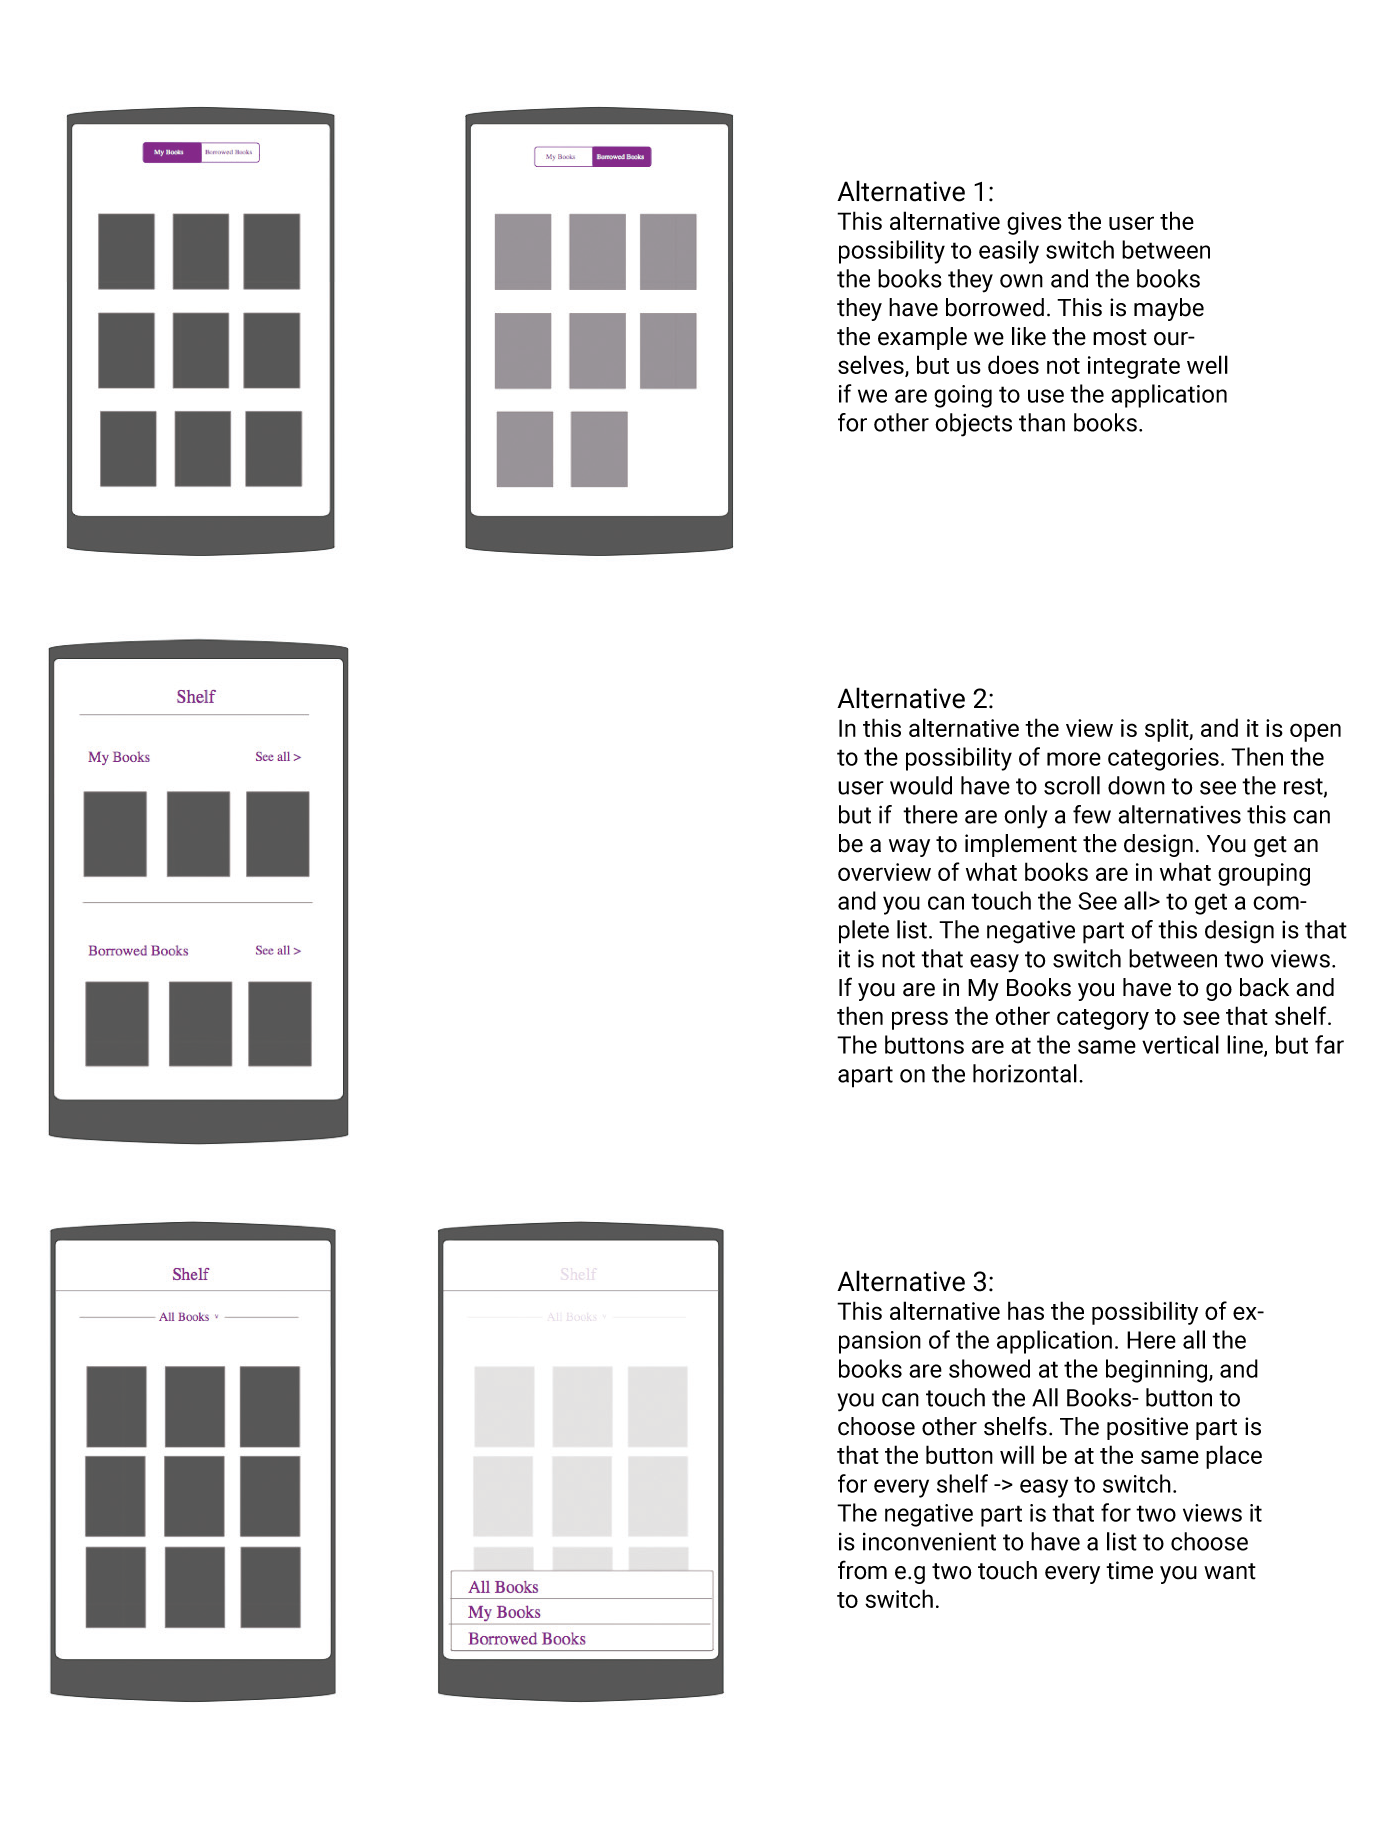
\includegraphics[height=22cm]{figs/v02/design-alternatives.png}
\caption{Design alternatives of the shelf view with argumentation }
\label{fig:design-alternatives-v2}
\end{figure}

\newpage
\subsection{User stories}
\label{user-stories-v2}
This section shows the user stories selected as requirements version 0.2. The stories are selected based on the initial assumption, and what was thought to be the most relevant features to test it. 

\begin{enumerate}
  \item As a user I want to add books to my shelf
  \item As a user I want to remove books from my shelf
  \item As a user I want to see the books in my shelf \label{02-user-story-see-books-in-shelf}
  \item As a user I want to search for books by scanning the barcode 
  
\end{enumerate}


\subsection{Development}
After the paper prototypes were done and had received feedback from users, the client teams started implementing the applications. Based on the user stories derived from the assumption and the prototype testing, the development team had enough information about what should be implemented to start the development. This section explains the implementation performed for this version in detail divided in sections of the subteams. 

\subsubsection{Android}
\begin{description}
    \item[Features] \hfill\\
The first feature the Android team developed for the Android application was the ability to scan a barcode of a book using the camera of an Android device to retrieve the ISBN number of a book. This was done by including a barcode image processing library called ZXing ("zebra crossing").\cite{zxing} The feature to be implemented was to retrieve information from this ISBN. This was done by sending an asynchronous \gls{HTTP} GET message to the Google Books' \gls{API} using the URL "http:www.googleapis.com/books/v1/volumes?q=isbn:", where the ISBN is concatenated to the end of the URL.\cite{http-method-spec} Since the call was asynchronous it could be executed in the background while the application could do other operations. If the Google Books contained information about the book, it would return the information stored in a JSON-object.\cite{json} Then Google's Java library GSON was used to convert the received JSON-object to Java objects.\cite{gson} This allowed the rest of the application to easily access the retrieved information and the team also chose to store this information in a local database called Realm. Realm stored the information locally, which meant that the next time the same information was needed it could be retrieved from Realm instead of performing another asynchronous request to Google Books. Realm, the local database, makes the information accessible to all activities and fragments of the application. Realm worked the same way with information retrieved from our \gls{backend}, where it stored information about books locally. The application also had to update the \gls{backend} when some changes were made, i. e. when a book was added or deleted.\\

\item[Structure] \hfill\\
The first version of the Android application contained many different classes since features such as networking and user interface was implemented. Figure \ref{fig:Android-structure-0.2} shows how the application's activities and fragments interacted. The \code{MainTabbedActivity} is the main activity launched when the application starts for the first time. This activity contains two tabs which are switching between displaying the two fragments \code{UserScreenFragment} and \code{ScannerScreenFragment}. The \code{UserScreenFragment} shows which books the user have stored, and the \code{ScannerScreenFragment} has the ability to scan barcodes using the camera of the device running the application. Information and data such as a barcode number in fragments are sent back to the \code{MainTabbedActivity}, which can start other activities using intents. 

The application communicates with the \gls{backend} and Google Books using a static class called \code{MainController}. This is explained further in chapter \ref{chap:ArchitecturalDescription}. 

\begin{figure}
\centering
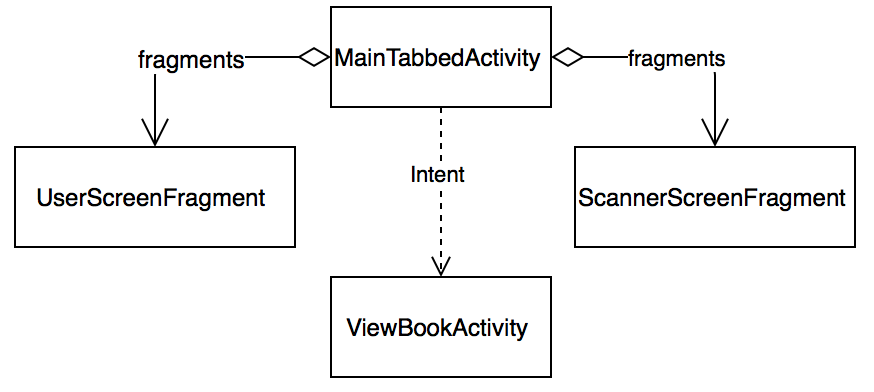
\includegraphics[width = \textwidth]{figs/v02/AndroidStructure02.png}
\caption{The structure of activities and fragments in the Android application in version 0.2}
\label{fig:Android-structure-0.2}
\end{figure}

\item[Design] \hfill\\
When the implementation of the functionality of version 0.2 was almost done, the Android team started looking at the usability of the application. Since none of the team members had much prior experience with Android development, they decided to set the basics of the design before to much code were implemented. The main activity was implemented as a tabbed activity. This made the activity able to have tabs that could be used to change between fragments, in addition to making it possible to swipe between fragments. This gives more possibilities to the design of the application, and the number of tabs could be set to one, to get it back to how it was. But in hindsight the team decided that version 0.2 should probably just be as basic as possible, focusing on implementing features. This would mean some extra work, but also more time to get feedback. Other than the tabbed activity this version was very basic. The elements were just placed somewhere they could be seen and used, but the sizes and relative locations were not important. The activity which shows book information and allows users to remove and delete books is shown in Figure \ref{fig:book-view-v2}.

\begin{figure}
\centering
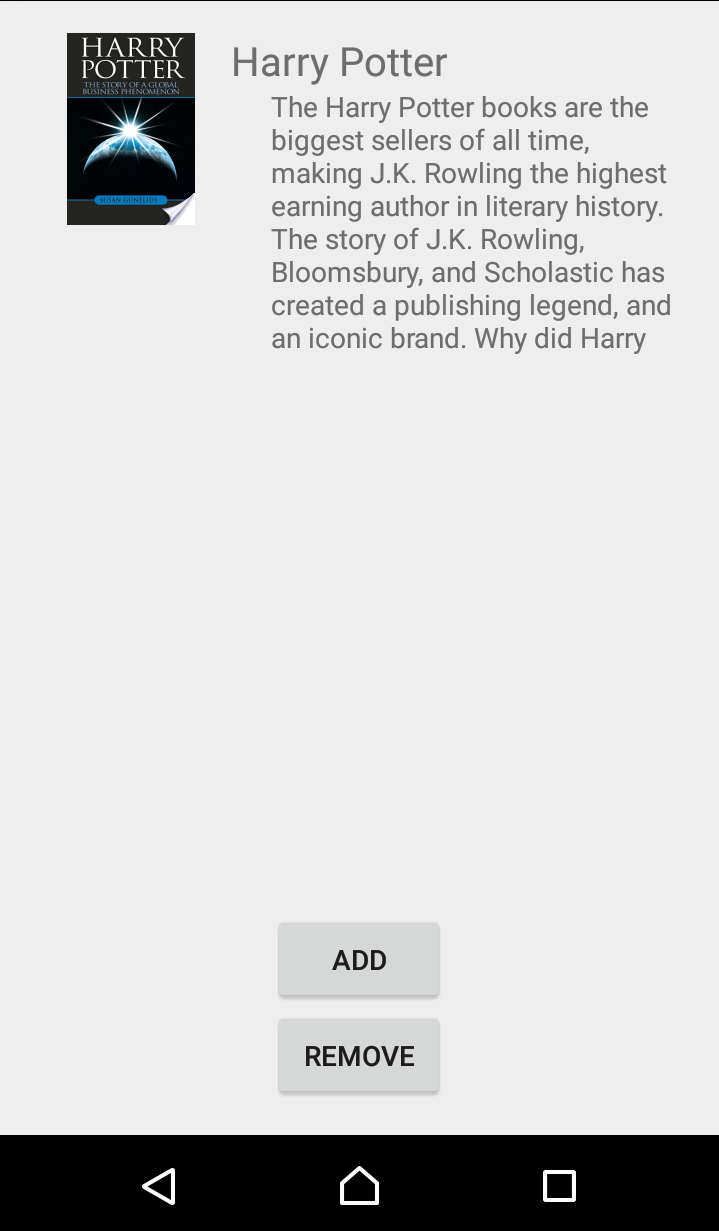
\includegraphics[height=7cm]{figs/v02/bookView02.png}
\caption{The ViewBookActivity showing book information in version 0.2 of the application}
\label{fig:book-view-v2}
\end{figure}

\item[User feedback] \hfill\\
To get feedback about how the users used the application, the analytics tool Mixpanel\cite{mixpanel} was added to the application. Using Mixpanel allowed the application to track specific actions the user performed. In version 0.2 Mixpanel registered each time a user launched the application and when a book was added. See table \ref{tab:mixpanel_table} for a full list of events that got tracked during version 0.2.
\end{description}

\subsubsection{iOS}
\begin{description}
\item[Structure] \hfill\\
This version was essentially a continuation of what the iOS team had been creating during version 0.1. It had been concluded that using the \gls{MVC} architectural pattern in combination with \gls{MVC} was the best approach.\cite{architectural-pattern} As most of the views, controllers and models were already created, the existing implementation only needed some minor changes. 

\item[Features] \hfill\\
The new feature in this release was that the application should communicate with the \gls{backend} when adding and removing books. This lead to the implementation of a new network handler class using the Alamofire library.\cite{alamofire} The network handler provided an interface for asynchronous \gls{HTTP} request for retrieval of information such as book and users. It would first try to parse the response as \gls{JSON}, but if that failed, it would treat the response as raw text. 

\item[Design] \hfill\\
The design used during the usability test was modified based on the feedback from users, and implemented in the application. The basic navigation method was iOS' standard tab bar, and all elements in the view conformed to Apple's Human Interface Guidelines. \cite{human-interface-guidelines} This was to ensure that all users would recognize the function of all elements such as buttons, labels and lists.

\item[User feedback] \hfill\\
In order to receive feedback from actual users about how they used the application, the iOS team integrated Mixpanel.\cite{mixpanel} It was used to track how users scanned books, added books, and removed books from their shelf. This was to be used when measuring the effect of future updates. Increased usage would indicate that the users were enjoying the application more than before the update.
\end{description}

\subsubsection{Backend}
The second iteration of the \gls{backend} was mostly spent improving upon the work from the first one. Everything was up on running, but there was no validation, and limited number of HTTP-response codes returned. In other words the server and \gls{API} was too simple, and the iteration was spent improving upon it. The team rewrote some of the \gls{API} endpoints and the data to be saved and returned, and added more context to responses and request. E.g. the team implemented the use of the HTTP-codes 404 and 422 to indicate that resources weren't present, or that a posted resource was on an invalid format. The team also implemented extensive validation of \gls{JSON}-data that was posted to the server. As a document-oriented database system lets you put anything into it, you have to enforce a data schema in the software code if you want it. This is why the team implemented the library Joi to validate the data. \cite{node-joi-module} This improved the communication with the client development teams.

The team also found that the server wasn't as RESTful as the team wanted it to be. It seems that the team misunderstood some of the aspects of the RESTful standards, which in turn meant that the team read up on it, and redesigned the API. \cite{w3c-rest} The team used the White House standard for RESTful APIs as a template, and used the APIs of GitHub and Twitter as inspiration. \cite{whitehouse-api-standard}\cite{github-api}\cite{twitter-api} Until now the only documentation of the \gls{API} was the readme-file in our project folder, available on GitHub. The latest version of the readme can be read in appendix \ref{app:backend-readme}. The customer wanted us to document the \gls{API} with Swagger, a tool to create an interface for your API, so that developers can explore it and easier understand it. \cite{swagger} First the team explored how the team could make the services already made self-documenting, but found that the tools to make an already exciting solution in Node self-documented with Swagger was hard. Instead the team wrote a Swagger specification with the Swagger Editor, that could be viewed in the Swagger UI. \cite{swagger-editor}\cite{swagger-ui} The Swagger-file written in the Swagger Editor was simply a \gls{YAML}-file on the format that the Swagger-UI needs. A screenshot of how the Swagger documentation looks in the Swagger UI, can be seen in figure \ref{fig:02swagger-docs}

The iteration also involved a lot of bug fixing, bugs that the client development teams reported over the course of the iteration.

\begin{figure}
\centering
\begin{subfigure}{\textwidth}
  \centering
  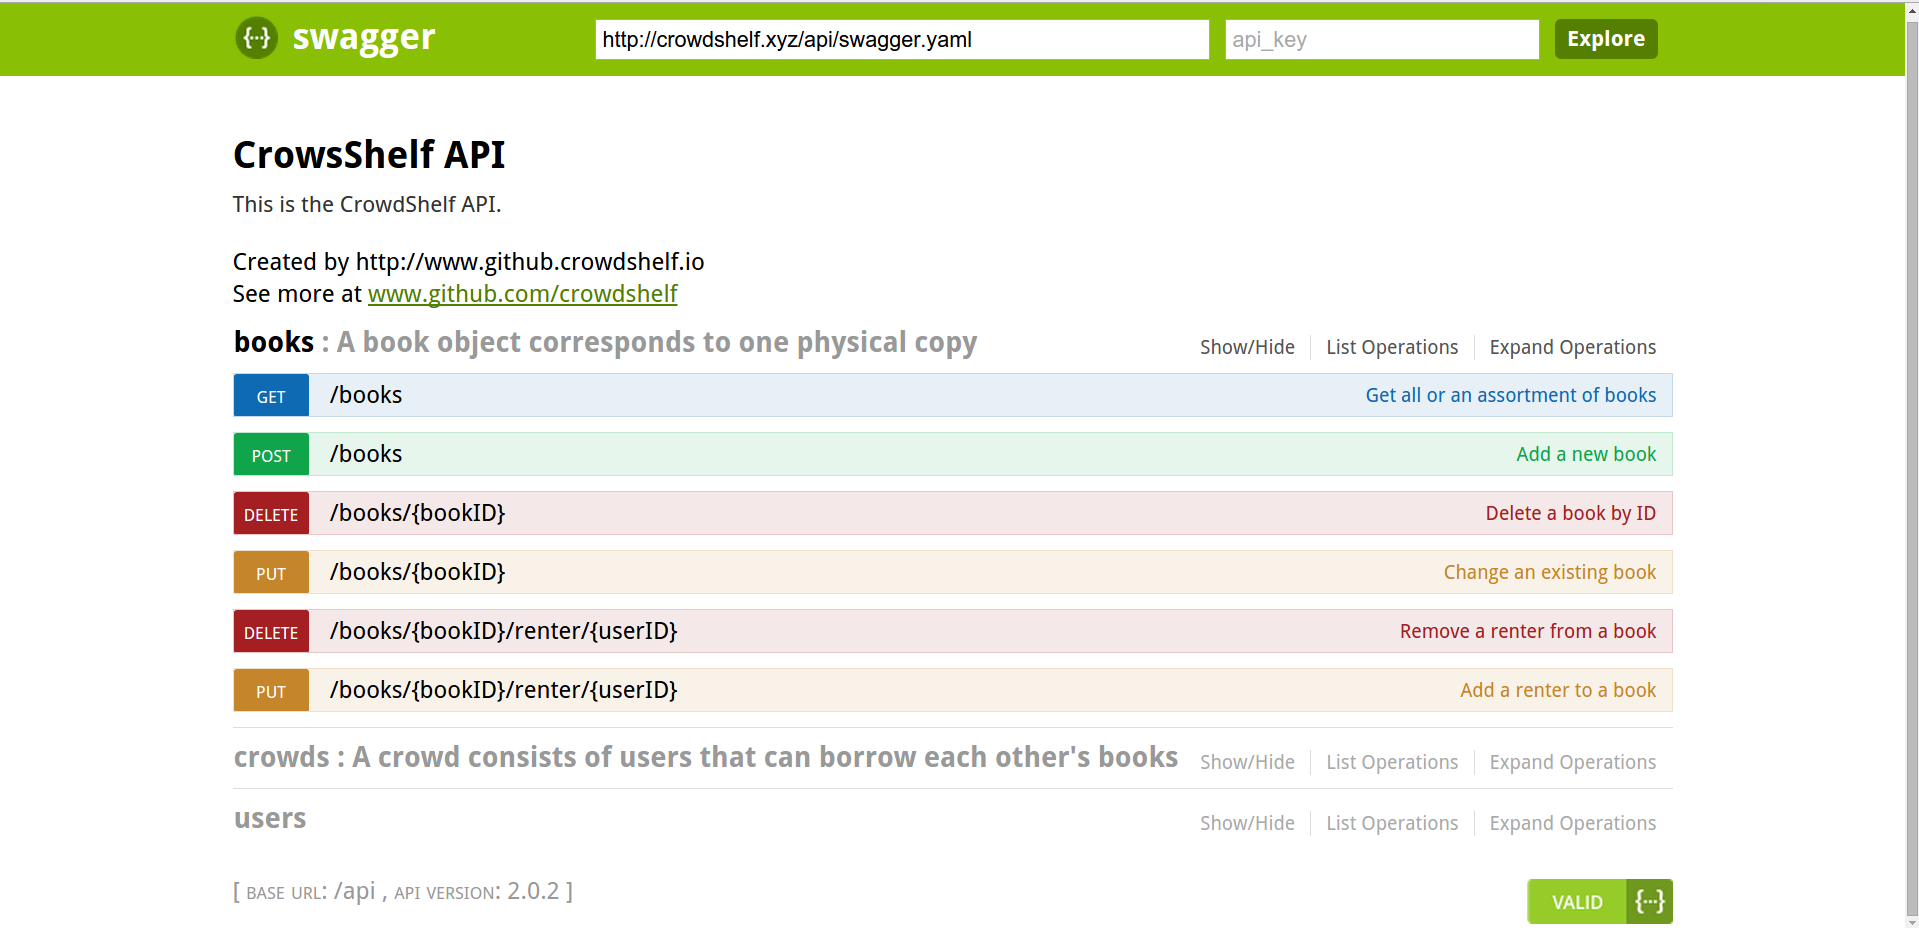
\includegraphics[width=\textwidth]{figs/v02/swagger2.png}
  \caption{Swagger with an overview of requests related to a specific entity.}
  \label{fig:swagger2}
\end{subfigure}%

\begin{subfigure}{\textwidth}
  \centering
  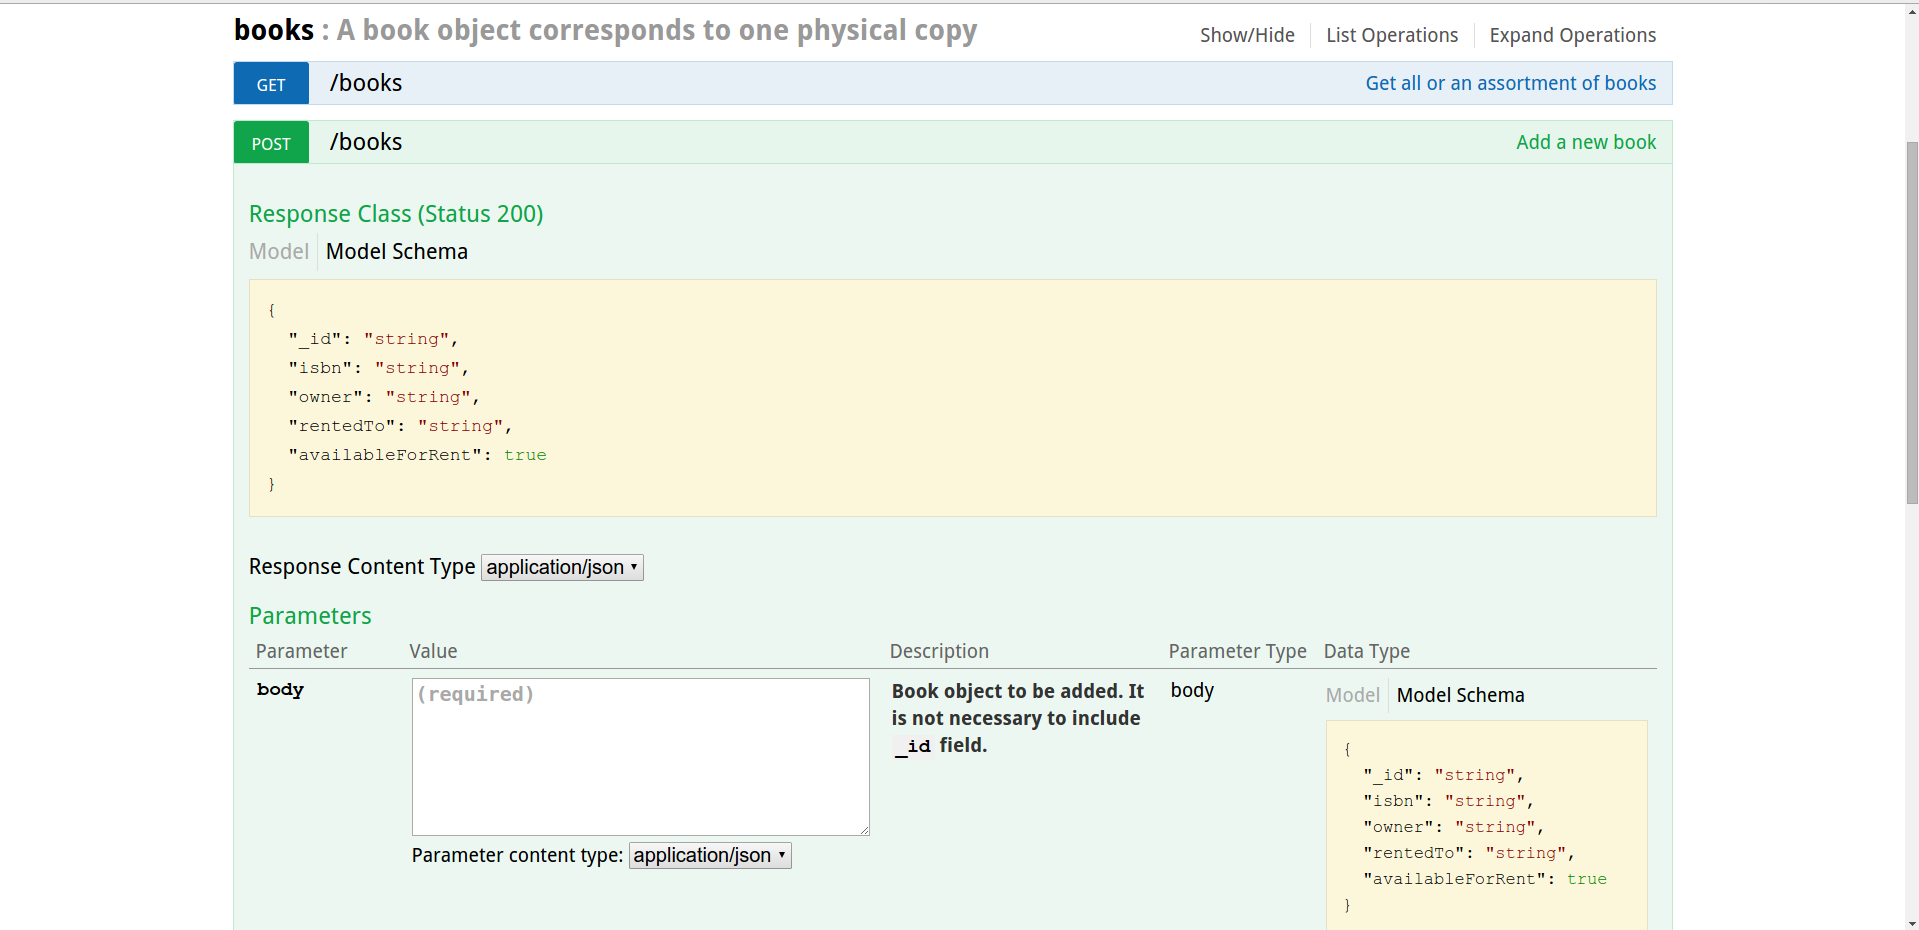
\includegraphics[width=\textwidth]{figs/v02/swagger3.png}
  \caption{Swagger when looking at a specific request.}
  \label{fig:swagger3}
\end{subfigure}
\caption{Screenshots from Swagger UI with the CrowdShelf \gls{API} specification}
\label{fig:02swagger-docs}
\end{figure}
\subsection{Feedback}

The feedback from the usability tests gave a positive indication that users would find it simple to add a book using a barcode scanner. Of the four users that were tested, three managed the tasks asked to complete without any trouble. The fourth subject had some trouble understanding the concept of the application, and as a consequence did not manage all the tasks without feeling very insecure in its use.

A few features of the application was mentioned to be improved. The users missed clear feedback when an action was taken, also the response was that the scanner button was easier to find if it was written scanner in contrast to an icon representing a camera. 

The finished version was sent to a few Netlight employees and students, but they were barely used. The customer representative was pleased with the increased velocity of the development, but this version was not yet ready to be used internally in Netlight. 

However, the team had received positive feedback regarding the features and usability of the application. Therefore it was decided to continue with the scanner solution and focus on the functionality chosen for the next version of the product. 

During this version a Facebook-page was also created to try to reach out to more users. The page gets updated every time a new version is released, and it contains a link to the project’s web page and to the Android application’s download page in Google Play. 

\subsection{Version progress}
As a consequence of the long duration of version 0.1, where no application was released, this version was completed very rapidly. In spite of a few obstacles, it took merely four days to complete four user stories with related 24 sub-tasks. As illustrated in figure \ref{fig:version-progress-2}, most tasks were completed on Monday and Wednesday when the whole team were working together. 

The release note found in appendix \ref{app:release-note-2} also show the consequence of a long first version iteration. Many of the tasks needed to complete the implementation of the applications were already completed before version 0.2.

The blog post used to describe the progress to the customer and supervisor are found in figure \ref{fig:week-five}.

\begin{figure}
\centering
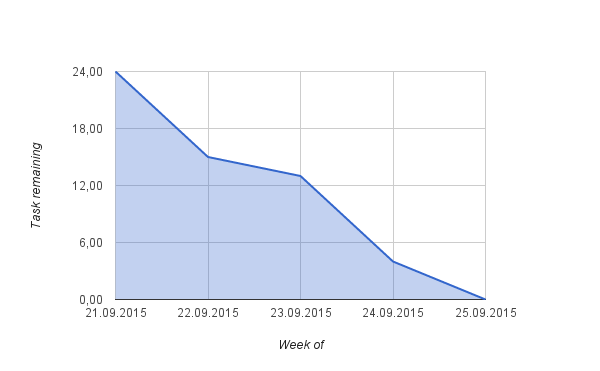
\includegraphics[height=10cm]{figs/v02/version-progress.png}
\caption{Task progression version 0.2}
\label{fig:version-progress-2}
\end{figure}

\begin{figure}
\centering
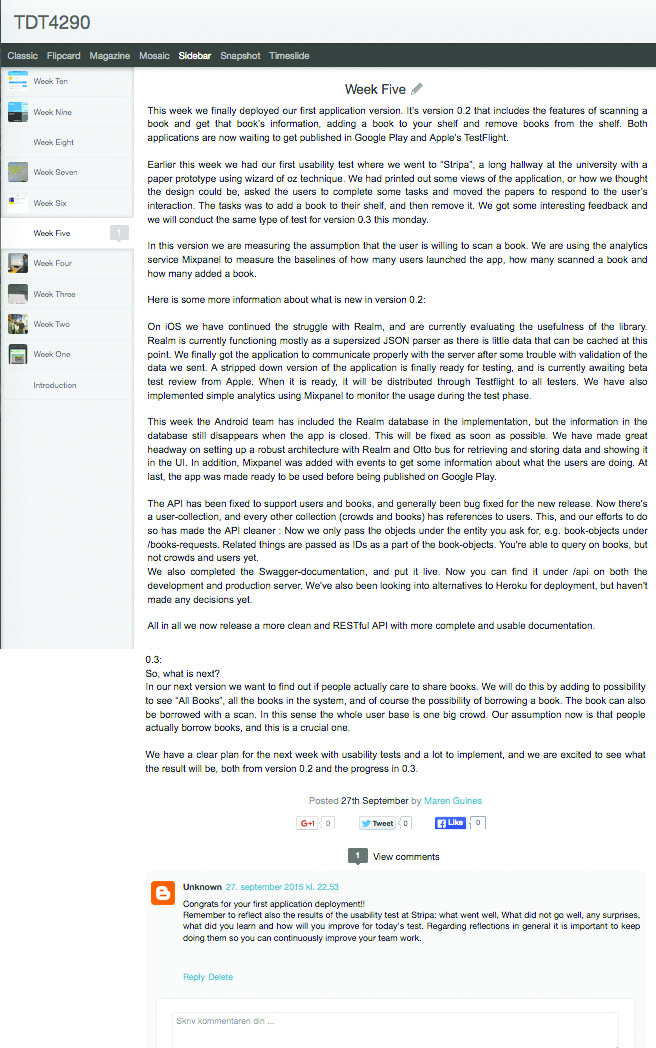
\includegraphics[height=22cm]{figs/v02/WeekFive.jpg}
\caption{Blog post from week 39}
\label{fig:week-five}
\end{figure}


\subsection{Review and retrospective}

At the customer meeting that was held during the second version, the team and the customer representative discussed the development progress. The customer representative stated that he missed the efforts he had seen the first weeks. The development had slowed down because of a lot of technical issues concerning the development of the Android application. Nevertheless, the team and the customer discussed possibilities to improve the progress. Increased use use of Netlight employees as support to the Android team would be an important factor in this effort. 

In addition, the customer representative had some input on what should be done before the next meeting. The design guidelines for iOS and Android should be studied, and a video of the application was to be shown at the next meeting.

One week later the customer representative was pleased with the development and the videos presented to show the functionality of the application. He always has a lot of feedback for the team to work on, and the team appreciates all his ideas and suggestions.

When the version was released, the team had a retrospective meeting where the overall atmosphere was positive. Communication within the team was mentioned under “What went well in this version”, as well as the fact that the application was released within the predetermined date. On the improvement side the team members mentioned the issue of having clear goals, and being able to work towards those goals. This will be the main focus point to try to improve in the next version.

Minutes from the costumer meeting is located in appendix \ref{app:customer-minutes-5}.

\subsection{Summary}
With the release of this version, it was possible to scan books to add and remove them from your virtual library, and browse all the books registered in the system.

Through usability tests an initial indication on the validity of the versions assumption was received, and a design of the functionality of the application version 0.2 was created.

The applications were completed on time and distributed through Google Play and TestFlight. Unfortunately the app was not downloaded enough to get any useful data from users this version either. The customer representative, who represent a lot of users in Netlight, seemed pleased with the results of the iteration.
